\documentclass[conference]{IEEEtran}
\IEEEoverridecommandlockouts
% The preceding line is only needed to identify funding in the first footnote. If that is unneeded, please comment it out.
\usepackage{cite}
\usepackage{amsmath,amssymb,amsfonts}
\usepackage{algorithmic}
\usepackage{graphicx}
\usepackage{textcomp}
\usepackage{xcolor}
\def\BibTeX{{\rm B\kern-.05em{\sc i\kern-.025em b}\kern-.08em
    T\kern-.1667em\lower.7ex\hbox{E}\kern-.125emX}}
\begin{document}

\title{A Method with Partial Hessian for Deep Recommendation System Optimization}


\author{\IEEEauthorblockN{1\textsuperscript{st} Gorkem Yencak} \\
%\IEEEauthorblockA{\textit{dept. name of organization (of Aff.)} \\
%\textit{name of organization (of Aff.)}\\
%City, Country \\
%email address or ORCID}
\and
\IEEEauthorblockN{2\textsuperscript{nd} Emre Sefer}}
%\IEEEauthorblockA{\textit{dept. name of organization (of Aff.)} \\
%\textit{name of organization (of Aff.)}\\
%City, Country \\
%email address or ORCID}}

\maketitle

\begin{abstract}
Second-order optimization algorithms have proven to be highly effective in solving traditional optimization problems, which has led to growing interest in adapting these methods for training deep neural networks (DNNs). However, a major challenge arises from the extremely high dimensionality of intermediate representations in DNNs, making the direct calculation and storage of the Hessian matrix impractical. Many earlier second-order optimization approaches rely on rough approximations of the Hessian, often leading to inconsistent results. In this project, we introduce a hybrid optimization method that merges a second-order optimizer—utilizing an accurate partial Hessian matrix for updating parameters at the channel level—with a first-order optimizer, specifically stochastic gradient descent (SGD), for updating all other parameters. We demonstrate that the Hessian matrices corresponding to channel-wise parameters are diagonal and can be computed accurately using Hessian-free techniques. Our method, called SGD with Partial Hessian for Deep Recommendation Systems~(SPHDRS), combines the strengths of both first-order and second-order optimization strategies. It leverages select Hessian information to enhance optimization over standard first-order methods, while maintaining the strong generalization ability that second-order methods often lack. Experimental results on both synthetic data and real-world recommendation system tasks confirm the effectiveness of SPHDRS.
\end{abstract}

%\begin{IEEEkeywords}
%Deep Learning, Second-order Optimization
%\end{IEEEkeywords}


\section{Introduction}

Thanks to the back-propagation algorithm, it is relatively straightforward and computationally efficient to obtain the first-order local information—such as gradients—of the loss function in deep neural networks (DNNs). This accessibility has significantly contributed to the widespread success of first-order optimization methods for training DNNs. Among these methods, Stochastic Gradient Descent with Momentum (SGDM) [1], [2] stands out as one of the most commonly used, relying solely on gradient information to determine the direction of descent. First-order optimizers [1]–[3] dominate DNN optimization due to their ease of implementation, low computational demands, and minimal memory usage. As expected, they have demonstrated strong performance across a range of tasks in computer vision [4], [5], natural language processing [6], and other areas of machine learning [7], [8].

In addition to first-order information, second-order information—such as the Hessian matrix—is widely recognized as potentially beneficial for optimization. In classical optimization problems, second-order algorithms are sometimes favored because they can achieve faster local convergence under certain conditions and reach higher accuracy with fewer iterations. As a result, extending second-order methods to optimize deep neural networks (DNNs) has remained an active area of research in recent years. However, a major challenge lies in the extremely high dimensionality of the Hessian in DNNs, making its direct computation and storage impractical. This makes the effective application of second-order methods in deep learning an unresolved issue.

Many studies have explored ways to approximate second-order information in DNNs. For instance, earlier research [9]–[11] has proposed Hessian-free techniques to estimate the Hessian and incorporate it into optimization. Yet, due to the limitations of these implementations, the approximated second-order information is often inaccurate, which may negatively affect the optimizer’s performance. Alternatively, some approaches focus on approximating the natural gradient—a different form of second-order information. Techniques like KFAC [12] and EKFAC [13] approximate the natural gradient by using a block-diagonal structure of the Fisher information matrix on a layer-by-layer basis. However, these methods rely on certain assumptions about the statistical behavior of parameter distributions, which can introduce further inaccuracies. Because of these factors, second-order optimizers can sometimes perform worse than their first-order counterparts, limiting their practical utility in deep learning applications.

It is important to highlight that most existing optimization algorithms treat all parameters in a neural network uniformly—that is, they apply the same update rule to every parameter during training. However, upon closer examination, we observe that certain one-dimensional (1D) channel-wise parameters frequently appear in widely used foundational components of deep neural networks, such as various normalization layers. From the perspective of optimizer design, we identify a valuable property of these 1D channel-wise parameters: the associated Hessian matrix for each group of them is diagonal (as shown in the derivation in Section II-A). Since the number of these parameters typically corresponds to the number of output channels in the layer—often a relatively small figure like 64—this makes it feasible to compute their diagonal Hessian entries both exactly and efficiently using Hessian-free techniques (refer to Section II-B for further explanation). This insight inspires a shift in perspective: instead of updating all parameters identically, we propose a new optimization strategy that selectively applies first-order or second-order methods, depending on the parameter type.

In this project, we propose a new type of compound optimizer, named SGD with Partial Hessian for Deep Recommendation System (SPHDRS), which combines the second-order optimizer for the channel-wise 1D parameters with the first-order optimizer for other parameters. Through making use of the special structure we mentioned above, we are allowed to use Newton-type methods to update parameters for some specific layers, such as the batch normalization (BN) layer and the convolutional layer with weight normalization (WN). Compared with first-order optimizers, SPHDRS adopts partial but precise information from the Hessian matrix to help optimization, while compared with other second-order optimizers, it can keep and even surpass the high generalization performance of first-order optimizers in recommendation tasks. Numerical experiments on different recommendation datasets are given to illustrate the effectiveness of our SPHDRS.

\subsection{Related Work}

When employing second-order methods for DNNs, an essential part is to consider how to extract the Hessian information efficiently and precisely. In this section, we list some Hessian-free methods for solving the descent directions. Besides, we also give a brief introduction of several commonly used normalization methods that inspire our design.

\begin{enumerate}
  \item Hessian-free Approaches: Hessian-free methods are intuitive and efficient in solving the descent direction when applying the Newton-type methods in DNNs optimization. Owing to the advantages of saving storage space, they are super suitable for deep networks and large-scale tensors. One kind of the Hessian-free method approximates the diagonal Hessian elements via back-propagation, e.g., the implementation process in Adahessian [11] and Apollo [9]. Specifically, Adahessian applies Hutchinson's method as an inexact approximation with the help of Rademacher distribution, and Apollo updates the descent direction by the quasi-Newton method with the help of the weak secant equation, in which the weak secant equation provides a reasonable diagonal approximation of the next Hessian matrix. Another kind is a generalization of the classical iterative methods, including the Gauss-Seidel method, the (preconditioned) conjugate gradient (CG) method, and the generalized minimal residual (GMRES) method. These well-known methods can iteratively solve the linear system without storing the whole Hessian matrix, and have also been embedded into the neural network training pipeline, e.g. [10], [14].
  \item Normalization Approaches: In DNNs, there are many specific layers designed to be channel-wise, which enables some good properties for designing a partial Hessian optimizer. The most intuitive examples are the batch normalization (BN) [15] and weight normalization (WN) [16]. BN is a usually adopted technique in high-level tasks training. In BN layers, a pair of parameters ( $\gamma, \beta$ ) is introduced to scale and shift the normalized value by $y_{i}=\gamma \hat{x}_{i}+\beta$ for each channel, such that the effect of noise will be reduced. By adding BN, the performance of many DNNs become more robust to the change of hyperparameter values. Differently, WN is a technique that decouples the length and the direction of the weight parameters, i.e., in mathematics, let $w=\gamma \frac{v}{l l v l l}$. By applying the WN method, we are able to decouple the weight length $\gamma$ and the direction tensor $v$ from the weight $w$. Without calculating statistics from mini-batches like BN, WN is more suitable for some specific applications such as deep reinforcement learning or generative models. Numerous experiments have confirmed that they can both speed up the training process and improve the final generalization performance. Besides WN and BN, there are also other feature normalization methods such as layer normalization (LN) [17], group normalization (GN) [18] and instance normalization (IN) [19]. Although these normalization layers are simple affine layers, they have a great favorable impact on training deep neural networks, which makes them become popular basic modules in DNNs.
\end{enumerate}


\section{Methodology}

Instead of using the overall first-order or second-order information, we design the descent steps with different order information at different layers, which is the reason we call our method a "partial Hessian" method. Here, based on the widely applied first-order optimizer SGDM, we add the precise Hessian information when optimizing the 1D parameters. Moreover, for DNNs that have no normalization layers, we can decouple the convolutional layers into a convolution operation and a linear weight normalization operation, which enables our optimizer to be applied. Here, we use Figure 1 to illustrate our idea.

\subsection{Diagonal Hessian Matrix}

For an intuitive explanation, we adopt the BN layer as an example to describe the design of SPH-DRS. For a BN layer, the 1D-parameters are formed by different values of parameters related to different channels. First we recall the operations of a single BN layer with C input channels. For a batch of input $X \in R^{N \times C \times W \times H}$ to this layer, divide it into $C$ sets $X_{1}, \ldots, X_{C}$ according to the channels, where $X_{i}=$ $\left\{x_{i}^{1}, x_{i}^{2}, \ldots, x_{i}^{m_{i}}\right\}$ for each channel index $i \in\{1,2, \ldots, C\}$ and $m_{i}=N W H$ represents the number of the elements within the i-th channel. Then for a specific channel $X_{i}$, the BN layer contains the following operations:
%
\begin{gather*}
\mu_{X_{i}}=\frac{1}{m_{i}} \sum_{j=1}^{m_{i}} x_{i}^{j} ; \sigma_{X_{i}}^{2}=\frac{1}{m_{i}} \sum_{j=1}^{m_{i}}\left(x_{i}^{j}-\mu_{X_{i}}\right)^{2}  \tag{1}\\
\hat{x}_{i}^{j}=\frac{x_{i}^{j}-\mu_{X_{i}}}{\sqrt{\sigma_{X_{i}}^{2}+\epsilon}} ; y_{i}^{j}=\gamma_{i} \hat{x}_{i}^{j}+\beta_{i} \tag{2}
\end{gather*}

The parameters $\gamma_{i}, \beta_{i}$ introduced here are usually updated via back-propagation in the training process. Notice that the
BN layer actually normalizes each channel independently, which means the parameters $\gamma_{i}, \beta_{i}$ of $X_{i}$ are irrelevant to $\gamma_{j}$, $\beta_{j}$ of $X_{j}$ whenever $j \neq i$. Thus, denote $\Gamma=\left(\gamma_{1}, \ldots, \gamma_{C}\right)^{T}$ as the group of parameters $\gamma_{i}$ for all the $C$ channels, the Hessian with respect to $\Gamma$, denoted by $H_{\Gamma}$ here, is exactly a diagonal matrix. i.e.,

\begin{figure*}[!h]
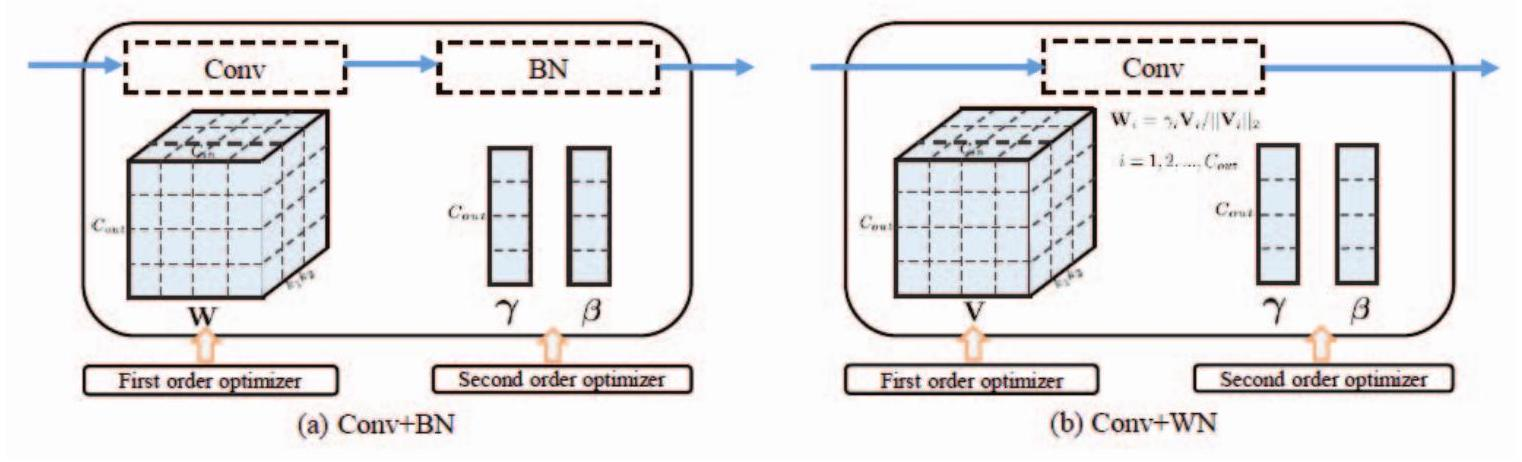
\includegraphics[scale=0.32]{figure1.jpg}
\caption{Illustration of SPH-DRS. Here, Figure (a) represents the case when BN is adopted in neural networks training, while other normalization methods such as LN, GN and IN can be represented in the same way. Figure (b) illustrates the case of decoupling the convolutional layers when there are no normalization layers followed, where $\beta$ represents bias, please see Section II-D for more details.}
\label{fig:1}
\end{figure*}

\begin{equation*}
H_{\Gamma}:=\frac{\partial^{2} L}{\partial \Gamma^{2}}=\operatorname{Diag}\left(\frac{\partial^{2} L}{\partial \gamma_{1}^{2}}, \ldots, \frac{\partial^{2} L}{\partial \gamma_{C}^{2}},\right) \tag{3}
\end{equation*}


with $\frac{\partial^{2} L}{\partial \gamma_{i}^{2}}=\sum_{j=1}^{m_{i}} \frac{\partial^{2} L}{\partial\left(y_{i}^{j}\right)^{2}}\left(\hat{x}_{i}^{j}\right)^{2}$ for $i=1, \ldots, C$. Then the inverse $H_{\Gamma}^{-1}$, if exists, can be computed directly by the inverse of each diagonal element. This structure states that getting the precise diagonal elements of the Hessian with respect to $\Gamma$ is equivalent to obtaining the partial Hessian $H_{\Gamma}$ precisely, which enables us to apply Newton-type methods easily. The same conclusion also holds for the Hessian of the group of parameters $\beta=\left(\beta_{1}, \ldots, \beta_{C}\right)^{T}$. Consequently, we can obtain the exact Hessian matrices of such one-dimensional parameters directly instead of using any approximation method.

It is worth mentioning that the property of partial diagonal Hessian does not hold for nature gradient descent methods (that is, the idea of extracting precise partial diagonal Hessian cannot be generalized to optimizers like KFAC), since the Fisher matrices related to 1D parameters are symmetric positive semidefinite matrices $E\left[g g^{T}\right]$ with $g$ being the gradient vector, which cannot be proved to be diagonal.

\subsection{The Hessian-free Approach}

As we mentioned in Section I-A, the Hessian-free method can be regarded as a necessary way in designing second-order optimizers due to the memory limitations, and some existing optimizers have adopted Hessian-free methods to approximate the whole Hessian diagonal. Under this situation, it seems that there is no need to extract the diagonal of some specific layers. However, regarding the truth that the whole Hessian is not diagonal, the inexactness brought by approximating the whole diagonal may influence the optimization process, which may lead to the unsatisfactory performance of the second-order optimizers on some tasks. As a consequence, by extracting the specific elements, we can avoid the inexactness of the existed diagonal approximation methods, which helps our optimization. In our optimizer, we adopt the Hessian-free approach with the help of back-propagation. To ensure continuity, we still take the BN layer as an example. Under the diagonal Hessian analysis Eq. 3, we set $e_{\Gamma}$ to be the vector that takes elements 1 related to the 1 D vector $\Gamma$ and takes elements 0 at all other places. Then with the help of the second time back-propagation, we can get
%
\begin{equation*}
H_{e_{\Gamma}}=\frac{\partial g^{T} e_{\Gamma}}{\partial \Gamma} \tag{4}
\end{equation*}
%
where $g$ is the gradient information computed in the first backpropagation process. Then the vector $\operatorname{diag}\left(H_{\Gamma}\right)$ is contained in the corresponding positions of the vector $H_{e_{\Gamma}}$. By this Hessian-free approach, we can get the corresponding diagonal matrix $H_{\Gamma}$ precisely without computing and storing the whole Hessian matrix. Hence, our method avoids the inaccuracy brought by the iterative methods or the approximation methods when computing the Hessian information. The analysis of the group of bias parameters $\beta$ in BN layers is the same as $\Gamma$. Apart from this, other normalization methods, including LN, IN and GN, also have analogous parameters, so similar derivations and conclusions can be obtained.

Generally, for an arbitrary 1D variable in DNN, we denote $e_{S O}$ the vector takes 1 at positions corresponding to this 1D vector and 0 at all other positions, and denote the partial diagonal Hessian matrix and the descent direction concerning it by $H_{S O}$ and $D_{S O}$, respectively. Figure 2 illustrates the idea of our precise diagonal Hessian computation. Through this operation, we can obtain the precise partial Hessian for the calculation of descent direction.

\subsection{Techniques in Nonconvex Optimization}

Since a nonconvex objective function may not have a positive-definite Hessian, to apply the Newton method in solving nonconvex stochastic optimization problems, several rectification techniques are usually adopted to guarantee the well-definiteness and the effectiveness of the Newton method.

\begin{figure}[!h]
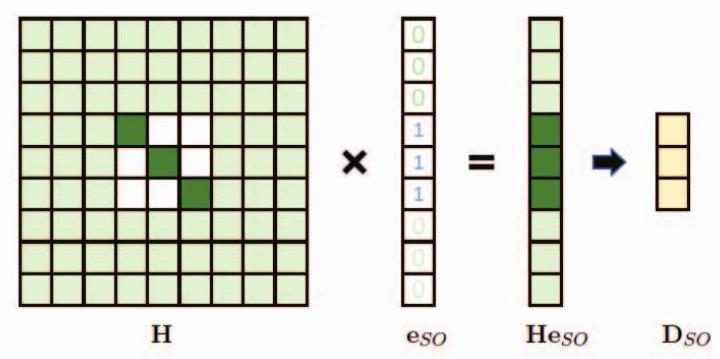
\includegraphics[scale=0.35]{figure2.jpg}
\caption{Illustration of diagonal Hessian computation. Here, the light green boxes represent the elements that can be any real numbers while the white boxes represent zeros. The central $3 \times 3$ matrix (i.e., $H_{S O}$ ) in $H$ is diagonal corresponding to the specific 1D variable. By multiplies with the vector $e_{S O}$, we can extract the diagonal elements precisely in the middle of $H e_{S O}$ and compute the element-wise inverse to get $D_{S O}$, which is exactly the diagonal of $H_{S}^{-1} O$.}
\label{fig:2}
\end{figure}

First, to handle the nonconvexity and noninvertible issues, we use the absolute value matrix with a positive perturbation as the substitution of the partial Hessian matrix, i.e.,
%
\begin{equation*}
\hat{H}_{S O}=\sqrt{H_{S O}^{T} H_{S O}}+\epsilon I \tag{5}
\end{equation*}


with $\epsilon>0$ a small enough positive real number. Moreover, at the $t$-th iteration, to minimize the effect of randomness and noise, we apply a momentum step on the Hessian information $\hat{H}_{S O}$, i.e., for some $\alpha \in(0,1)$, the momentum $M_{H}$ is computed by


\begin{equation*}
M_{H^{t}}=(1-\alpha) M_{H^{t-1}}+\alpha \hat{H}_{S O}^{t} \tag{6}
\end{equation*}


and the inverse of partial Hessian $D_{S O}^{t}=\left(\operatorname{diag}\left(M_{H^{t}}\right)\right)^{-1}$ is computed directly by taking the diagonal element-wise inverse. At each iteration $t$, we only calculate the partial Hessian and the momentum related to the current 1D parameter. The techniques we mentioned above are some generally used techniques that can also be found in many other papers about second-order optimizers, e.g., [9], [11].

Here, as applied in SGD, we also apply the momentum [2] calculation on the gradient and the weight decay [20] technique for the final descent direction in our optimizer to accelerate the convergence. Specifically, the momentum step on the gradient is


\begin{equation*}
M_{G^{t}}=(1-\beta) M_{G^{t-1}}+\beta \hat{G}^{t} \tag{7}
\end{equation*}


where $\beta \in(0,1)$ is a given constant and $G$ is the gradient of the parameters. Meanwhile, after computing the final descent direction $D_{G}$ (specifically, taking $D_{S O} M_{G}$ for 1D parameters and $M_{G}$ for the others), for a given weight decay parameter $\eta$ and the weight tensor $W$, the weight decay step is exactly


\begin{equation*}
\hat{D}_{G}^{t}=D_{G}^{t}+\eta W^{t} \tag{8}
\end{equation*}

%With the techniques in this section, we are ready to introduce the structure of our optimizer SGD with Partial Hessian for Deep Recommendation System (SPH-DRS) in Algorithm 1.

\subsection{Generalizations on Convolutional Layers}

In the previous sections, we explained how to apply SPHDRS to DNNs with normalization layers. In this section, we will suggest that our optimizer can also be applied in training DNNs without normalization layers in the same way of weight normalization (WN). Here we illustrate the derivation via a single 2D convolution operation $Y=W * X$, where $W$ is the kernel with dimension $C_{\text {out }} \times C_{\text {in }} \times k_{1} \times k_{2}$ and $X$ is the input. For each output channel $i \in\left\{1, \ldots, C_{\text {out }}\right\}$, the WN operation can be defined as follows:
%
\begin{equation*}
W_{i}=\gamma_{i} \frac{V_{i}}{\left\|V_{i}\right\|_{2}}, \text { where } V_{i} \in R^{C_{i n} \times k_{1} \times k_{2}} \text { and } \gamma_{i} \in R \tag{9}
\end{equation*}

Overall, we can get $V=\left(V_{1}, \ldots, V_{C_{\text {out }}}\right)$ and $\Gamma=$ $\left(\gamma_{1}, \ldots, \gamma_{C_{\text {out }}}\right)$. Thus, the parameters to be optimized change from the initial parameterW to the same dimension parameter $V$ and a channel-wised 1D parameter $\Gamma$. Similar to the parameters in BN, our proposed optimization algorithm can also be adopted to optimize the parameter $\Gamma$ with its secondorder information. Moreover, the bias parameter $\beta$ in the convolutional layers can also be contained into the secondorder part optimization of SPH-DRS (we omit the details since it is trivial).

\section{Experiments}

We will test the performance of SPH-DRS over DLRM which is one of the state-of-the-art deep recommendation models, recently developed by Facebook [21]. We measure the performance of DLRM, which instead uses our method, in terms of Click Through Rate (CTR).

\subsection{Synthetic Datasets}

DLRM takes continuous and categorical attributes as its inputs. In this case, we model continuous attributes via random vector generation from either a Gaussian or uniform distribution. We model categorical attributes by first determining the number of non-zero items in a given multi-hot vectors where we follow a procedure similar to random data generation in [21].

\subsection{Real Datasets}

There are number of publicly-available datasets for personalization and recommendation systems. Among them, we will focus on 2 frequently-used datasets: Criteo Ad Kaggle [21] and Criteo Ad Terabyte [21]. Both datasets are composed of click logs for predicting ad click-through rate (CTR). Both datasets include 26 categorical and 13 continuous attributes. We preprocess the continuous attributes by using a simple logarithmic transformation $\log (1+x)$. We map each categorial attribute to its matching embedding index where we map unlabeled categorical attributes or labels to NULL or 0.

Among these datasets, the Criteo Ad Kaggle dataset incorporates almost 45 million sample points over a week period. In our experiments, we utilize the initial six days as the training set and the seventh day becomes the validation and test sets. On the other hand, The Criteo Ad Terabyte dataset instead covers samples over 24 days. In this case, all days except the last day compose the training set whereas we partition the last day into validation and test sets. In both datasets, we observe almost equal number of sample points for each day.

\subsection{Performance Evaluation}

We validate the robustness and effectiveness of our proposed SPH-DRS by comprehensive experiments on recommendation system tasks. In our experiments, we compare our method with first-order optimizers SGDM [2], Adam [1], AdamW [22], Adabelief [3], together with second-order optimizers Adahessian [11] and Apollo [9]. We tune the learning rate and weight decay for all these methods, and choose their best results for comparison. Specifically, the learning rates are set to be 0.1 for SGDM, 0.001 for Adam, AdamW and Adabelief, 0.15 for Adahessian and 1 for Apollo. The weight decays are set to be 0.0005 for SGDM, Adam and Adahessian, 0.5 for AdamW and Adabelief, and 0.00025 for Apollo.

In SPH-DRS, the hyperparameters $\alpha$ and $\beta$ control the momentum for the partial Hessian matrix and the gradient, respectively. Following the experience from SGDM, we set $\alpha=0.9$ and $\beta=0.9$ in our experiments. The second-order learning rate $\tau_{S O}$ in line 7, Algorithm 1 is set to be 0.001 . Besides, we add a small positive number $\epsilon=0.0001$ to the Hessian diagonal to avoid the diagonal elements being zero. Our experiments are accomplished on Pytorch 1.7 framework with mainly TITAN RTX and Geforce RTX 2080Ti GPUs. The batch size, learning rate, and weight decay will be introduced in each section.

\section{Results}

\subsection{Synthetic Dataset Results}

In our experiments on synthetic datasets, we train DNNs with different optimizers for total 200 epochs, using batch size 128 with one single GPU, and the learning rate is multiplied by 0.1 every 60 epochs. For all optimizers including SPH-DRS, we utilize 2 approaches to schedule learning date decay: 1Milestone strategy which decreases the learning rate at the end of predetermined epochs, 2- Cosine annealing strategy which is discussed in [22].

According to Table I, we find that our SPH-DRS outperforms all competing approaches. Especially, the performance of SPH-DRS surpasses other compared methods largely. The performance of SPH-DRS surpasses SGD, which fully indicates that the precise partial Hessian can help improve the final performance. We notice that many optimizers (e.g., SGDM, Adabelief, Apollo and SPH-DRS) reach $100 \%$ training accuracy with loss near to zero, so most of them show quite similar generalization performance as in Table I. In the meantime, we also find that the performance of Adahessian sometimes is not stable, e.g., its performance in all four synthetic scenarios drops largely. The imprecise Hessian adopted in Adahessian sometimes may have very bad impacts on the optimization process.

\begin{table}[!h]
\centering
\begin{tabular}{ccccc}
\hline
 & \multicolumn{2}{c}{Gaussian} & \multicolumn{2}{c}{Uniform} \\
Method & Milestone & Cosine & Milestone & Cosine \\
\hline
SGDM & $89.8 \pm 1.8$ & $90.0 \pm 2.1$ & $89.9 \pm 2.2$ & $90.2 \pm 2.2$ \\
Adam & $90.2 \pm 1.5$ & $90.7 \pm 1.5$ & $90.4 \pm 1.8$ & $90.5 \pm 1.7$ \\
AdamW & $90.4 \pm 1.4$ & $90.6 \pm 1.6$ & $90.5 \pm 1.5$ & $90.7 \pm 2.3$ \\
Adabelief & $91.1 \pm 1.7$ & $92.3 \pm 2.1$ & $91.5 \pm 1.6$ & $91.8 \pm 2.9$ \\
Adahessian & $90.7 \pm 1.7$ & $91.1 \pm 1.7$ & $91.0 \pm 1.8$ & $91.2 \pm 1.6$ \\
Apollo & $91.5 \pm 1.9$ & $91.3 \pm 1.1$ & $90.9 \pm 2.1$ & $91.4 \pm 1.9$ \\
SPH-DRS & $92.5 \pm 3.5$ & $92.9 \pm 2.5$ & $92.4 \pm 3.1$ & $92.8 \pm 2.9$ \\
\hline
\end{tabular}
\caption{Testing accuracies (\%) on synthetic datasets generated by using gaussian and uniform distributions. Performance of two learning rate schedulers are compared: Milestone and Cosine.}
\end{table}

\section{Performance on Real Criteo Ad Datasets}

In our real experiments, we evaluate the performance of our optimizer SPH-DRS on modern recommendation systems, especially on DLRM that is quite frequently used in the literature [21]. Those systems incorporate a big embedding layer which is accompanied by a sequence of dense Fully Connected (FC) Layers. In training, a sparse set of rows of the embedding layer is used and only those rows are updated. These rows do change from one iteration to the next. For such a sparse setting, we use SPH-DRS to update the embedding table, as well as update the rest of the FC network in the experiments. As seen in Table II, the testing accuracy of SPH-DRS is $79.167 \%$, which is $0.62 \%$ higher than the best performing competing method. It should be noted that this is a quite significant accuracy increase for Recommendation Systems [23].

\begin{table}
\centering
\begin{tabular}{ccc}
\hline
Method & Criteo Ad Kaggle & Criteo Ad Terabyte \\
\hline
SGDM & $77.92 \pm 0.58$ & $78.08 \pm 0.65$ \\
Adam & $78.22 \pm 0.68$ & $78.11 \pm 0.71$ \\
AdamW & $78.40 \pm 0.74$ & $78.35 \pm 0.75$ \\
Adabelief & $78.44 \pm 0.49$ & $78.22 \pm 0.48$ \\
Adahessian & $78.52 \pm 0.59$ & $78.41 \pm 0.69$ \\
Apollo & $78.55 \pm 0.61$ & $78.44 \pm 0.73$ \\
SPH-DRS & $79.17 \pm 0.71$ & $79.05 \pm 0.82$ \\
\hline
\end{tabular}
\caption{Testing accuracy of SPH-DRS and a number of existing optimizers on Criteo Ad Kaggle and Criteo Ad Terabyte datasets.}
\end{table}

\begin{enumerate}
  \item Time and Memory Cost: To extract the precise partial Hessian information without approximation, the Hessian free method via the second time back-propagation is the best approach for SPH-DRS. In Adahessian, the same technique has also been applied, and sadly the time consumption and the storage cost increase exaggeratedly (e.g., for Criteo Ad Kaggle dataset, Adahessian has 4.64 times increase in time and 1.30 times increase in storage compared to SGDM), which may result in a bad impact on its comprehensive applications. By noticing this fact, we have optimized the calculation process in our Hessian-free approach due to our special structure to shorten the time and storage cost of the second time backpropagation. Although we still have increments of 2.22 and 1.23 times in time and storage respectively compared to SGDM due to the properties of back-propagation, we have saved the time and storage a lot compared to Adahessian that adopting the same technique.
\end{enumerate}

\section{Ablation Studies}

In this section, we will report some ablation studies about SPH-DRS to state its robustness and efficiency. We first tune some important hyperparameters, including the initial learning rate, weight decay, the second-order learning rate and the momentum of partial Hessian, then we test the performance of SPH-DRS under different input batch size settings. Similarly, we repeat each experiment 4 times and report the results in the mean $\pm$ standard deviation format.

\begin{enumerate}
  \item Learning Rate and Weight Decay: Generally, good settings for learning rate and weight decay can greatly benefit the final generalization results. In our experiments, we choose the learning rate (LR) and weight decay (WD) from the set $\{0.005,0.01,0.02\}$, while the learning rate of the secondorder part $\tau_{S O}$ and the Hessian momentum $\alpha$ are set to be 0.001 and 0.9 , respectively. Table III shows the results of five combinations of LR and WD. We found the best result by setting LR to be 0.01 and WD to be 0.005 , and we adopt this in the experiments of Section IV-B. Moreover, other settings also achieve acceptable results with fluctuations of no more than $0.77 \%$ and $0.83 \%$ for Criteo Ad Kaggle and Criteo Ad Terabyte datasets respectively, which illustrates that SPH-DRS is robust to these hyperparameters.
  \item Batch Size: The input batch size can also affect the performance of optimizers. Hence, we also pay attention to the impact of different batch size on the performance of SPHDRS. Here, we provide Table IV about the testing accuracy\\
results of SPH-DRS for both Criteo Ad Kaggle and Criteo Ad Terabyte datasets, with the hyperparameters settled by $l r=0.01, w d=0.005, \tau_{S O}=0.001$ and $\alpha=0.9$. When the batch size increases from 16 to 256 , there is a certain range of fluctuations in the testing accuracies, with the best result occurring at batch size 32 for both datasets. Totally, the trend of fluctuation about SPH-DRS related to batch size is similar to other widely used optimizers, which ensures the adaptability and stability of SPH-DRS for different settings in applications.
  \item Second-order Learning Rate: In SPH-DRS, an additional important hyperparameter is imported, i.e., the learning rate of the second-order part $\tau_{S O}$. Here we tune $\tau_{S O}$ on both Criteo Ad Kaggle and Criteo Ad Terabyte datasets by traversing through the set $\{0.01,0.001,0.0001\}$, while the initial LR and WD are set to be 0.01 and 0.005 , respectively. Table V gives the testing accuracies of different $\tau_{S O}$ on those datasets. We can see from the results that, on Criteo Ad Kaggle dataset, a smaller $\tau_{S O}$ (i.e., 0.0001) may achieve better generalization performance. Meanwhile, on Criteo Ad Terabyte dataset, the performances of SPH-DRS with different $\tau_{S O}$ have no significant differences. Thus, the results in Table V shows the applicability of our proposed SPH-DRS related to different second-order LR $\tau_{S O}$. Furthermore, as a moderate choice, we take the hyperparameter $\tau_{S O}=0.001$ in the above sections, and it works well through all of our experiments.
  \item Hessian Momentum: Following the experience of tuning the momentum of SGDM, we list some testing accuracy results of SPH-DRS with different Hessian momentum parameters $\{0.8,0.9,0.99\}$ for both Criteo Ad Kaggle and Criteo Ad Terabyte datasets in Table VI. As shown in Table VI, $\alpha=0.9$ attains the best results (which is the value we adopt in the previous sections), while other parameters also achieve acceptable results with a maximum fluctuation of $0.24 \%$ and $0.76 \%$ for Criteo Ad Kaggle and Criteo Ad Terabyte datasets respectively. Consequently, SPH-DRS performs stably with these commonly chosen values of momentum.
\end{enumerate}

\section{Conclusions}

In this paper, we propose SPH-DRS, a compound optimizer that combines first-order optimizer SGDM with partially accurate Hessian information. The design of SPH-DRS is based on the derivation of the Hessian matrices of the channel-wise 1D parameters, which are proved to be diagonal matrices and can be extracted precisely through the Hessian-free method. Besides showing the effectiveness of SPH-DRS on various synthetic recommendation datasets, we also evaluate its performance on two real recommendation datasets. Sufficient ablation studies are accomplished to verify the robustness and adaptability of our proposed SPH-DRS related to different hyperparameters. However, consistent with other second-order optimizers, our SPH-DRS also needs more computational time and memory compared with first-order optimizers. This is still one of the key problems faced for designing second-order optimizers.

\begin{table*}[!h]
\centering
\begin{tabular}{cccccc}
\hline
LR & 0.01 & 0.01 & 0.01 & 0.02 & 0.005 \\
\hline
WD & 0.01 & 0.002 & 0.005 & 0.005 & 0.005 \\
\hline
Criteo Ad Kaggle & $79.19 \pm 0.45$ & $79.33 \pm 0.14$ & $\mathbf{7 9 . 9 6} \pm \mathbf{0 . 3 0}$ & $79.21 \pm 0.20$ & $79.28 \pm 0.28$ \\
Criteo Ad Terabyte & $80.05 \pm 0.28$ & $80.21 \pm 0.16$ & $\mathbf{8 0 . 8 8} \pm \mathbf{0 . 2 4}$ & $80.08 \pm 0.35$ & $80.48 \pm 0.21$ \\
\hline
\end{tabular}
\caption{Testing accuracies (\%) of different LR and WD for both Criteo Ad Kaggle and Criteo Ad Terabyte datasets.}
\end{table*}

\begin{table}
\centering
\begin{tabular}{cccccc}
\hline
Batch Size & 16 & 32 & 64 & 128 & 256 \\
\hline
Criteo Ad Kaggle & $79.38 \pm 0.38$ & $\mathbf{7 9 . 8 1} \pm \mathbf{0 . 3 3}$ & $79.58 \pm 0.18$ & $79.07 \pm 0.11$ & $78.78 \pm 0.31$ \\
Criteo Ad Terabyte & $80.31 \pm 0.25$ & $\mathbf{8 0 . 6 8} \pm \mathbf{0 . 2 2}$ & $80.28 \pm 0.28$ & $79.88 \pm 0.34$ & $79.22 \pm 0.20$ \\
\hline
\end{tabular}
\caption{Testing accuracies (\%) of different batch size settings for both Criteo Ad Kaggle and Criteo Ad Terabyte datasets.}
\end{table}

\begin{table*}[!h]
\begin{tabular}{cccc}
\hline
$\tau_{S O}$ & 0.01 & 0.001 & 0.0001 \\
\hline
Criteo Ad Kaggle & $79.21 \pm 0.23$ & $79.77 \pm 0.34$ & $\mathbf{8 0 . 1 6} \pm \mathbf{0 . 3 0}$ \\
Criteo Ad Terabyte & $79.77 \pm 042$ & $80.35 \pm 0.20$ & $\mathbf{8 1 . 0 2} \pm \mathbf{0 . 4 5}$ \\
\hline
\end{tabular}
\caption{Testing accuracies (\%) of different second-order learning $\tau_{S O}$ for for both Criteo Ad Kaggle and Criteo Ad Terabyte datasets.}
\end{table*}

\begin{table}[!h]
\centering
\begin{tabular}{cccc}
\hline
$\alpha$ & 0.8 & 0.9 & 0.99 \\
\hline
Criteo Ad Kaggle & $79.72 \pm 0.24$ & $\mathbf{7 9 . 9 6} \pm \mathbf{0 . 3 0}$ & $79.89 \pm 0.51$ \\
Criteo Ad Terabyte & $80.12 \pm 0.18$ & $\mathbf{8 0 . 8 8} \pm \mathbf{0 . 2 4}$ & $80.45 \pm 0.29$ \\
\hline
\end{tabular}
\caption{Testing accuracies (\%) of different $\alpha$ for both Criteo Ad Kaggle and Criteo Ad Terabyte datasets.}
\end{table}

\begin{thebibliography}{00}
\bibitem{b1} G. Eason, B. Noble, and I. N. Sneddon, ``On certain integrals of Lipschitz-Hankel type involving products of Bessel functions,'' Phil. Trans. Roy. Soc. London, vol. A247, pp. 529--551, April 1955.
\bibitem{b2} J. Clerk Maxwell, A Treatise on Electricity and Magnetism, 3rd ed., vol. 2. Oxford: Clarendon, 1892, pp.68--73.
\bibitem{b3} I. S. Jacobs and C. P. Bean, ``Fine particles, thin films and exchange anisotropy,'' in Magnetism, vol. III, G. T. Rado and H. Suhl, Eds. New York: Academic, 1963, pp. 271--350.
\bibitem{b4} K. Elissa, ``Title of paper if known,'' unpublished.
\bibitem{b5} R. Nicole, ``Title of paper with only first word capitalized,'' J. Name Stand. Abbrev., in press.
\bibitem{b6} Y. Yorozu, M. Hirano, K. Oka, and Y. Tagawa, ``Electron spectroscopy studies on magneto-optical media and plastic substrate interface,'' IEEE Transl. J. Magn. Japan, vol. 2, pp. 740--741, August 1987 [Digests 9th Annual Conf. Magnetics Japan, p. 301, 1982].
\bibitem{b7} M. Young, The Technical Writer's Handbook. Mill Valley, CA: University Science, 1989.
\end{thebibliography}

\end{document}
